\section{Метод решения}
Метод спектрального угла относится к методам классификации с обучением. Данное семейство методов предполагает наличие эталонов, 
с которыми сравнивается каждый пиксель. В результате, имея несколько эталонов, заранее заданных, мы имеем множество объектов, 
разделенных на классы. Для метода спектрального угла нам понадобится представить каждый пиксель в виде вектора и 
вычислить угол между текущим пикселем и эталлоным пикселем. В качестве результирующего класса для пикселя выбирается класс, 
имеющий наименьший угол между текущим и эталлоным пикселем.

Алгоритмическая сложность алгоритма --- $O(n \cdot w \cdot h)$, где $n$ -- количество классов.
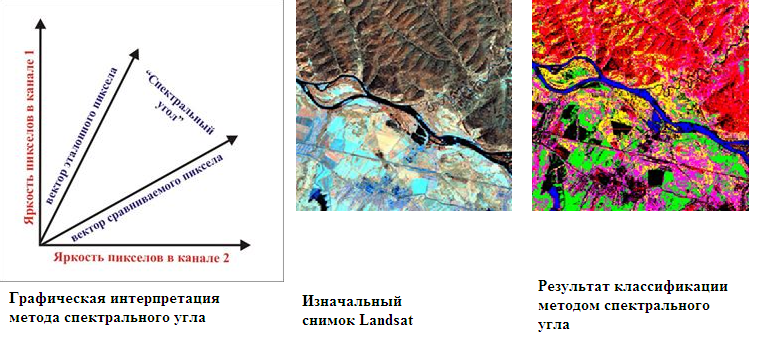
\includegraphics[scale=0.7]{spec_angle}

\section{Описание программы}
Проект я разделил на следущие модули:
\begin{enumerate}
    \item $common \; defines$ - содержит множество полезных дефайнов для более приятной работы с $CUDA$ и $C++$.
    \item $common \; structures$ - содержит класс-обертку над $CUDA$ событиями и класс-обертку над $std\!::\!stringstream$, позволяющим конструировать строки ($sprintf$ с возможностями $C++$).
    Также сюда были помещены классы-обертки над текстурными объектами и ресурсами.
    \item $operation \; system$ - содержит операции, связанные с системными вызовами (например, получение информации о количестве оперативной памяти). Реализован только для ОС $Windows$.
    \item $claster$ - содержит класс кластера, имеющий методы для чтения и вычисления среднего значения.
    \item $kernel$ - непосредственно программа, выполняющия все операции, связанные с вводом, вычислениями и выводом.
\end{enumerate}

Также для замера времени была написана программа на языке программирования $Python$, состоящая из слеудющих модулей:
\begin{enumerate}
    \item $build$ используется для компиляции $Microsoft\:Visual\:Studio$ проекта (файла с расширением $.sln$).
    \item $tests \; generator$ используется для генерации тестов и ответов на них (ответы генерируются с помощью программы, написанной под $CPU$).
    \item $cheker$ используется для проверки работоспособности программы.
     Для этого запускается раннее сгенерированный $.exe$ файл с входными данными из теста, далее вывод программмы проверяется с ответом.
    \item $benchmark$ используется для замера скорости работы программы. Для этого программа запускается 5 раз с входными тестовыми данными.
     Для каждого теста временем работы будет минимальное время работы из всех запусков данного теста.
    \item $converter$ используется для конвертации изображения в бинарный вид и для получения изображения из бинарных данных.
    \item $main$ используется в качестве обертке над описанными выше модулями для более комфортного запуска модулей.
\end{enumerate}